\chapter{General Overview}
\abstract*{General}

\section{Description of Vegvisir Implementation}

The Vegvisir blockchain is a tamperproof log that can be shared among IoT
devices. The implementation is based on a membership protocol. The participants
are defined prior to creation of the blockchain.  This is also true concerning
the type of information that is shared. The set-up is differs slightly from the
instantiation of the database as fields and participants can be added after the
initial creation. The added rigidity of Vegvisir's protocol allows for
additional security and for streamlined type-based operations associated with
the applicable CRDT. The fundamental use of this blockchain is to ensure that
events that happen in a distributed system are securely logged. The protocol
has implications for food supply tracking, emergency response, food management
and much more.

%\begin{figure*}[!htbp]
\begin{wrapfigure}{L}{.45\textwidth}
    \centering
    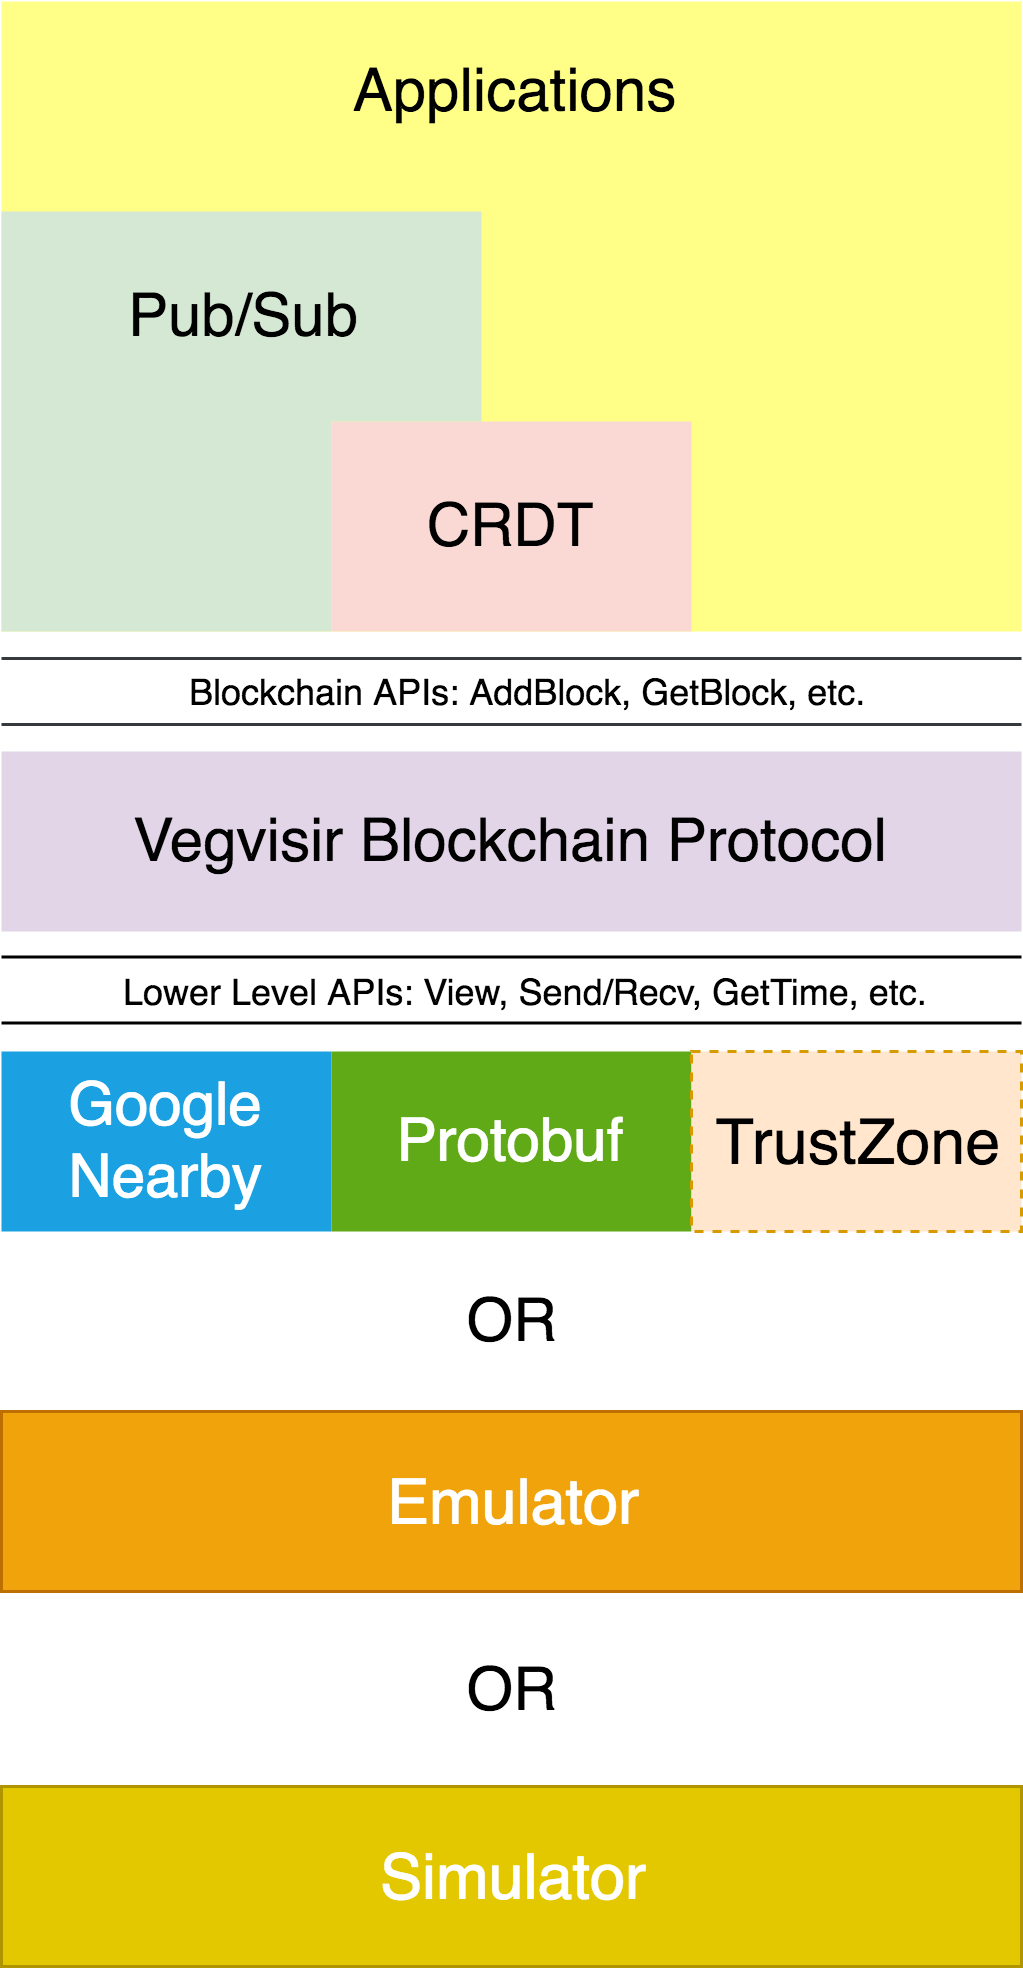
\includegraphics[scale=0.26]{Veg_Structure.png}
    \caption{Vegvisir Structure}
    \label{fig:structure}
\end{wrapfigure}
%\end{figure*}

The implementation can be broken down into three different sections:
\begin{enumerate}
    \item{ Core }
    \item{ Application layer }
    \item{ Lægra }
\end{enumerate}
Figure \ref{fig:structure} shows the overview of the system. The \emph{core} is
listed as "Vegvisir Protocol" in lavender. The application layer is above, and
Lægra is located below. Lægra, or "the lower", can be represented by Protobuf,
TrustZone, or any of the other included structures represented in tis section.

On either side the \emph{core}, there are API's. These are the approved
mechanisms for interacting with the \emph{core}. These will be defined in their
associated sections.
